\documentclass{article}
\usepackage{graphicx}
\usepackage{float}
\usepackage{latexsym}
\usepackage{amsfonts,amsmath,amssymb}
\usepackage{authblk}
\usepackage{url}
\newcommand{\hConds}{$20$}
\newcommand{\voConds}{$5$}
\newcommand{\vnConds}{$23$}
\newcommand{\vConds}{\vnConds{}}
\newcommand{\hTotal}{$1442$}
\newcommand{\hGlobal}{$473$}
\newcommand{\hGlobalLB}{$352$}
\newcommand{\hGlobalShuff}{$12$}

\newcommand{\hHorizIntercept}{$-0.36$}
\newcommand{\hHalflife}{$1.9$}

\newcommand{\vnTotal}{$1142$}
\newcommand{\voTotal}{$919$}
\newcommand{\vTotal}{\vnTotal{}}

\newcommand{\voGlobalShuff}{$152$}
\newcommand{\vnGlobalShuff}{$5$}
\newcommand{\vGlobalShuff}{\vnGlobalShuff{}}

\newcommand{\vnGlobal}{$305$}
\newcommand{\voGlobal}{$378$}
\newcommand{\vGlobal}{\vnGlobal{}}

\newcommand{\vnIntercept}{$-0.54$}
\newcommand{\voIntercept}{$-0.54$}
\newcommand{\vHalflife}{$1.29$}
\newcommand{\hProtsInRange}{$414$}
\newcommand{\vProtsInRange}{$221$}

\newcommand{\hMeanSlope}{$1.32$}
\newcommand{\hMeanSlopeStdDev}{$0.57$}
\newcommand{\hSlopeStdErrMean}{$0.34$}
\newcommand{\hRibsMeanSlope}{$1.41$}
\newcommand{\hRibsSlopeStdDev}{$0.32$}
\newcommand{\hRibsSlopeStdErrMean}{$0.23$}
\newcommand{\hGlobalSumSlope}{$1.24$}
\newcommand{\hGlobalSumRsq}{0.91}
\newcommand{\hRibsSumSlope}{$1.37$}
\newcommand{\hRibsSumRsq}{0.89}

\newcommand{\hRibs}{$53$}
\newcommand{\hCorrRibs}{$47$}

\newcommand{\vnRibs}{$53$}
\newcommand{\voRibs}{$54$}
\newcommand{\vRibs}{\vnRibs{}}
\newcommand{\vnCorrRibs}{$52$}
\newcommand{\voCorrRibs}{$52$}
\newcommand{\vCorrRibs}{\vnCorrRibs{}}

\newcommand{\vnMeanSlope}{$1.06$}
\newcommand{\voMeanSlope}{$1.39$}
\newcommand{\vMeanSlope}{\vnMeanSlope{}}

\newcommand{\vMeanSlopeStdDev}{$0.60$}
\newcommand{\vSlopeStdErrMean}{$0.14$}
\newcommand{\vRibsMeanSlope}{$1.48$}
\newcommand{\vRibsSlopeStdDev}{$0.08$}
\newcommand{\vRibsSlopeStdErrMean}{$0.06$}

\newcommand{\vnGlobalSumSlope}{$1.0$}
\newcommand{\voGlobalSumSlope}{$1.39$}
\newcommand{\vGlobalSumSlope}{\vnGlobalSumSlope{}}

\newcommand{\vnGlobalSumRsq}{0.97}
\newcommand{\voGlobalSumRsq}{1.0}
\newcommand{\vGlobalSumRsq}{\vnGlobalSumRsq{}}

\newcommand{\vnRibsSumSlope}{$1.49$}
\newcommand{\voRibsSumSlope}{$1.49$}
\newcommand{\vRibsSumSlope}{\vnRibsSumSlope{}}

\newcommand{\vnRibsSumRsq}{0.97}
\newcommand{\voRibsSumRsq}{0.97}
\newcommand{\vRibsSumRsq}{\vnRibsSumRsq{}}

\newcommand{\hMaxExpVar}{0.082}
\newcommand{\vnMaxExpVar}{0.035}
\newcommand{\voMaxExpVar}{0.04}
\newcommand{\vMaxExpVar}{\vnMaxExpVar{}}

\title{Increased concentration of proteins with growth rate as a result of passive resource-redistribution}

\author{Uri Barenholz}
\author{Leeat Keren}
\author{Eran Segal}
\author{Ron Milo}
\affil{Weizmann Institute of Science}
\date{\vspace{-5ex}}
\bibliographystyle{plain}

\begin{document}

\maketitle 

\begin{abstract}
Changes in thousands of gene levels across conditions make it difficult to interpret “omics” studies and find causative explanations.
Can much of this variation result from passive redistribution of resources also affecting the growth rate? Following a review of previous efforts we suggest a simple model that predicts an increase in the fraction of many proteins out of the proteome, proportionally with the growth rate.
The model reveals how active regulation of only a few proteins can have proteome wide effects that are quantitatively predictable.
We exemplify the usage of the model with several recent proteomics data sets.
We find that many proteins from different cellular processes, far beyond the previously suggested group of ribosomal proteins, increase their fraction of the proteome proportionally with the growth rate.
Our model suggests a base-line null-model explaining these changes in expression levels across conditions.
\end{abstract}

\section{Introduction}
A fundamental system biology challenge is to understand and predict changes in gene expresssion levels. In the last two decades, with the ability to measure genome-wide expression levels, there is an avalanche of new data and a need for principles and models to facilitiate their interpretation. Early on it was found that ribosome concentration increases in proportion to the specific growth rate \cite{Schaechter1958}.
The observed increase in concentration has been interpreted as an increased need for ribosomes at faster growth rates \cite{Neidhardt1999,Dennis2004,Zaslaver2009,Molenaar2009}.
The search for underlying mechanisms in \emph{E.coli} yielded several candidates \cite{Nomura1984} such as the pools of ppGpp and iNTP \cite{Murray_2003,Bosdriesz_2015}, and the tRNA pools through the stringent response \cite{Chatterji2001,Brauer2008a}.

More recetly, it was found that changes in gene expression as a function of growth rate are not limited to ribosomal genes.
In \emph{E.coli}, the expression of catabolic and anabolic genes is coordinated with growth rate, and suggested to be mediated by cAMP \cite{Saldanha2004,You_2013,Peebo_2015}.

In \emph{S.cerevisiae}, it was shown that most of the genome changes its expression levels in response to environmental conditions in a manner strongly correlated with growth rate \cite{Keren2013a,Brauer2008,Castrillo2007,Gerosa2013}.
Studies examining the interplay between global and specific modes of regulation, suggested that global factors play a major role in determining the expression levels of genes \cite{Gasch2000,Klumpp2009,Klumpp2014,Scott2010,Berthoumieux2013,Keren2013a,Gerosa2013,Valgepea2013,Hui_2015}.
In \emph{E.coli}, this was mechanistically attributed to changes in the pool of RNA polymerase core and sigma factors \cite{Klumpp2008}.
In \emph{S.cerevisiae}, it was suggested that differences in histone modifications around the replication origins \cite{Regenberg2006} or translation rates \cite{Brauer2008} across conditions may underlie the same phenomenon.
Taken together, these studies suggest that the expression of all genes changes with growth rate, with different factors and architectures of regulatory networks yielding differences in the direction and magnitude of these changes \cite{Klumpp2009,Klumpp2014}. 

Despite these advancements, our ability to predict expression levels across conditions remains limited.
Here we present a parsimonious model that quantitatively predicts the relationship between protein abundance and specific growth rate in the absence of gene-specific changes in regulation.
Our model provides a baseline for the behavior of genes in conditions between which they are not differentially regulated, without the need for condition-specific parameters.
The model predicts an increase in protein expression with specific growth rate as an emerging property that is the result of passive redistribution of resources, without need for specific regulation mechanisms.
On top of this baseline model, different regulatory aspects, that are definitely at play, can be added.
We tested the model against recently published proteomic data sets of \emph{E.coli} spanning different growth conditions \cite{Valgepea2013,Peebo_2015,Heinemann2015}.

We find a coordinated, positive correlation between the specific growth rate and the fraction of many proteins, from diverse functional groups, out of the proteome.
Although this response accounts for a relatively small part of the total variability of the proteome it is highly relevant for understanding proteome wide studies, as it describes the behavior of about $50\%$ of the proteome genes.
The well-studied ribosomal proteins are found to be a small subset of this group of proteins that increase their fraction with the specific growth rate.
Our analysis suggests that, even if changes in the proteome composition are complex, for a large number of proteins and under many conditions such changes take the form of a linear, coordinated, increase with growth rate.
An increase that can result from cellular reources being freed by down-regulated proteins.
The well studied scaling of ribosome concentration with growth rate can be considered one manifestation of this more general phenomena.

\section{Results}

\subsection{Simple considerations predict passively driven increase in the fraction of proteins as a function of the specific growth rate}

What is the simplest way to model the differences in the proteome composition of two populations of cells, one growing in a permissive environment, and the other facing a more challenging growth condition?
In an attempt to parsimoniously analyze such differences, we have constructed a minimalistic model that predicts the behavior of non-differentially regulated genes across different growth conditions.
Before presenting the model mathematically, we give a brief intuitive depiction.

The model assumes that under a favorable growth condition, the cell actively down-regulates some proteins that are only needed in harsher conditions, as illustrated in Figure \ref{fig:model}.
The down regulation of the lac operon in the presence of glucose is a prominent example for this phenomenon.
As a result of only that specific change, the fraction of all other proteins out of the proteome is increased compared to the harsher (e.g. growth on lactose) condition.
In our baseline model, all the other proteins increase their levels and are expected to show the same relative ratios between each other in all conditions.
Specifically, the proteins forming the bio-synthetic machinery increase their levels and therefore their fraction out of the proteome.
Thus, the ratio of the bio-synthetic machinery to the proteome increases.
The growth rate is dependent on the amount of protein bio-synthesis a cell performs.
The increase in ratio of bio-synthetic machinery to proteome thus results in an expected increase in the growth rate, as depicted in Figure \ref{fig:model}.
In our example of the lac operon, in the presence of glucose, the down regulation of lactose metabolism genes leads to faster growth as more bio-synthetic genes are expressed instead.

\begin{figure}[H]
\begin{center}
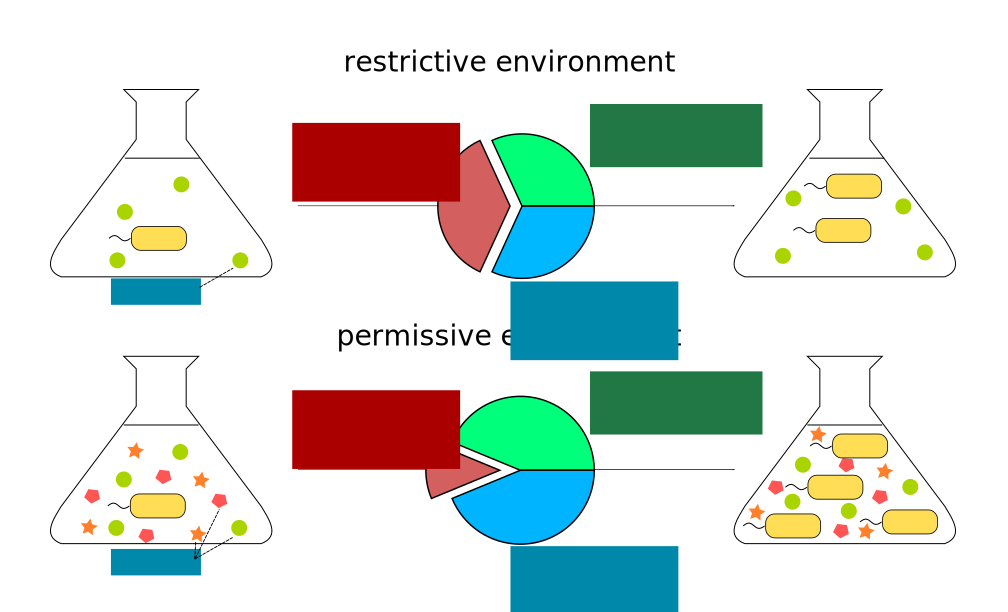
\includegraphics[width=\columnwidth]{../figure1.pdf}
\caption{\label{fig:model}
A minimalistic model predicts that low expression of condition-dependent genes under permissive growth environment, compared with a restrictive environment, implies larger fraction of all other proteins out of the proteome.
With this, the ratio of bio-synthesis genes to the rest of the proteome is higher in permissive environments, resulting in faster growth.
%
}
\end{center}
\end{figure}

\subsubsection{The expression level of a protein can be decomposed into gene specific control and global
expression machinery availability}

The composition of the proteome can in principle be determined by a large number of parameters.
For example, given that an organism expresses 1000 genes across 10 different growth conditions, one could imagine that controlling the expression pattern of all genes across all conditions will require 10,000 parameters.
Our model proposes an underlying architecture that drastically reduces this amount of parameters, implying that cells control most of the composition of their proteome through fewer degrees of freedom than might be naively expected.

The model separately considers the resulting fraction of every protein out of the proteome as the product of two control mechanisms: 
\begin{enumerate}
\item Protein/gene specific controls which only affect the individual protein under a given condition.
These include the gene associated promoter affinity, 5'-UTRs, ribosomal binding site sequence, as well as the presence of transcription factors and riboswitches that react with the relevant gene.
We note that while a given transcription factor may affect many genes, the presence or absence of its relevant binding sequence is gene specific, making this control mechanism gene specific in the context of our analysis.
  While some of these controls (such as the ribosomal binding sites) are static, and therefore condition independent, others are dynamic and will differ across different environmental conditions (such as transcription factors state, for genes that are affected by them).
\item Global expression control based on the availability of bio-synthetic resources, including RNA polymerase, co-factors, ribosomes, amino-acids etc.
  All of these factors can potentially differ across different environmental conditions and no gene can avoid the consequences of changes in them.
\end{enumerate}

In the model, every gene is given an 'affinity-for-expression' (or 'intrinsic-affinity') score that encapsulates its tendency to attract the bio-synthetic machinery, as was first suggested in \cite{Maaloe1969}.
This gene-specific value can in principle change across conditions but a key feature is that the gene intrinsic affinity tends to have the same value across many conditions.
Often two values are enough across all conditions, an "off" and "on" value.
We denote the affinity of gene $i$ under growth condition $c$ by $w_i(c)$.
To determine the resulting fraction of every protein, our model assumes that the bio-synthetic resources are distributed among the genes according to those affinities, as is stated in Equation \ref{eq:concentration-ratio}. Intuitively, one can think of a competition between the genes and transcripts over the bio-synthesic resources, where each gene/transcript attracts resources according to its intrinsic affinity.

The notion of intrinsic affinities represents the expression pattern under a given condition by the intrinsic affinities of all genes under that condition.
Assuming each gene has only a finite set of affinities, possibly only one or two (for example, on and off states of the lac operon), describing the expression pattern is therefore reduced to selecting which, out of the total gene-specific small set of possible affinities, each gene gets under the relevant condition.
Given that the selection of expression level for a given gene is driven by some specific environmental cues, the description can be further reduced to determining what cues are present at each condition.



The fraction of a specific protein out of the proteome is equal to the specific affinity of the corresponding gene under the condition, divided by the sum of the affinities of all genes under that same condition.
To illustrate: if two genes have the same affinity under some condition, their corresponding proteins will occupy identical fractions out of the proteome.
If gene $A$ has twice the affinity of gene $B$ under a given condition, then the fraction protein  $A$ occupies will be twice as large as the fraction occupied by protein $B$ under that condition, etc.

This relationship can be simply formulated as follows:
\begin{equation}
  \label{eq:concentration-ratio}
  p_i(c)=\frac{P_i(c)}{P(c)}=\frac{w_i(c)}{\sum_jw_j(c)}
\end{equation}
where $p_i(c)$ denotes the fraction out of the proteome of protein $i$ under condition $c$, $P_i(c)$ denotes the mass of protein $i$ under condition $c$ per cell, $P(c)$ denotes the total mass of proteins per cell under condition $c$, and the sum, $\sum_jw_j(c)$, is taken over all the genes the cell has.

This equation emphasizes that the observed fraction of a protein is determined by the two factors mentioned above: the specific affinity of the protein/gene, that is present in the numerator, and also, though less intuitive, the affinity of all other genes under the growth condition (affecting the availability of bio-synthetic resources), as reflected by the denominator.

For simplicity, the model refers to the fraction of each specific protein in the proteome and not to the protein concentration.
The corresponding concentration in the biomass can be calculated using the concentration of total protein in the biomass.
In \emph{E.coli}, this concentration is known to slightly decrease in a linear manner with the specific growth rate \cite{Bremer1987,Valgepea2013,Scott2014}.

\subsubsection{A change in growth condition triggers changes in expression of specific proteins that indirectly affect the whole proteome}
Different environmental conditions require the expression of different genes.
For example, the expression of amino-acids synthesizing enzymes is required only in culture media lacking amino-acids \cite{24656150,10515934}.
Therefore, the cell can infer the presence or absence of amino-acids in the growth media and, regulate the affinities of the synthesizing genes accordingly.
If we consider a gene $i$, whose specific affinity is not dependent on the presence of amino-acids, we suggest that its fraction will still change between the two conditions as the affinities of other condition specific genes change, thereby redirecting the bio-synthetic capacity.
In mathematical terms this will chang the denominator in equation \ref{eq:concentration-ratio} and thus affect the distribution of resources between all of the expressed genes.


Generalizing this notion, we can divide the proteins into those whose intrinsic affinity remains constant across all of the considered conditions, and those whose intrinsic affinity changes between at least some of the conditions (Figure \ref{fig:model}).
An interesting consequence is that proteins whose intrinsic affinities remain constant also maintain their relative ratios across these conditions with respect to each other, as observed experimentally in \emph{S.cerevisae} in \cite{Keren2013}.

\subsubsection{Growth rate is the combined outcome of proteome composition and environmental conditions}
While it is sometimes implied that different cellular components are regulated by the growth rate, our model considers the growth rate as an outcome of the environmental conditions that affect the proteome composition.
Specifically, we assume that the doubling time is proportional to the ratio of the total amount of proteins per cell and the proteins involved in bio-synthesis in that cell.
The larger the ratio of total proteins to bio-synthesis proteins is, the longer these bio-synthesis proteins will need to duplicate the proteome, resulting in a longer doubling time.

To illustrate this assumption concretely, one could think about the synthesis of polypeptides.
If a cell has $R$ actively translating ribosomes, each of which synthesizing polypeptides at a rate of $\eta \approx 20$ amino acids per second, the bio-synthetic capacity of the cell will be limited to $\approx \eta R$ amino acids per second.
If the total amount of protein in that same cell is $P$ (measured in amino acids count), it follows that the time it will take the actively translating ribosomes to synthesize the proteins for an identical daughter cell is $\tau \approx \frac{P}{\eta R}$ (up to a $\ln(2)$ factor resulting from the fact that the ribosomes also synthesize more ribosomes during the replication process and that these new ribosomes will increase the total rate of polypeptides synthesis).


The theoretical lower limit of the doubling time, $T_B$, will be achieved when all of the proteome of the cell is the bio-synthetic machinery.
If the bio-synthetic machinery is only half of the proteome, the doubling time will be $2T_B$ etc.

To integrate the notion of total protein to bio-synthetic protein ratio into our model, we make the following simplifying assumption:
There is a group of bio-synthetic genes (e.g. genes of the transcriptional and translational machineries) the affinities of which remain constant across different growth conditions, that is, these genes are not actively differentially regulated across different conditions.
Furthermore, we assume that the machineries these genes are involved in, operate at relatively constant rates and active to non-active ratios across conditions, as has been shown for ribosomes \cite{Bremer1987}.

Formally, we define the group of bio-synthesis genes, $G_B$, such that, for every gene that belongs to this group, $k \in G_B$, its affinity, $w_k(c)$ is constant regardless of the condition, $c$.
\begin{equation}
  \label{eq:biosynth-def}
  w_k(c)=w_k
\end{equation}

To keep our notations short, we will define the condition independent sum over all of these bio-synthesis genes as the constant:
\[
W_B = \sum_{k\in G_B}w_k
\]

The doubling time under a given condition, $\tau(c)$, will be proportional to the ratio of total protein to bio-synthesis protein under that condition, with the proportionality constant $T_B$:
\begin{equation}
  \label{eq:gr-ratio}
  \tau(c) = T_B\frac{P(c)}{\sum_{k\in G_B}P_k(c)}=T_B\frac{\sum_jw_j(c)}{W_B}
\end{equation}
Therefore, the model reproduces an increase in the doubling time for conditions requiring larger amounts of non-bio-synthetic proteins (i.e. higher values in the sum across $w_j$).

\subsubsection{The fraction of a non-differentially regulated protein is expected to increase with the growth rate} 
Recalling that the connection between the growth rate and the doubling time is: $g(c)=\frac{\ln(2)}{\tau(c)}$, we now combine Equation \ref{eq:concentration-ratio} with Equation \ref{eq:gr-ratio} to get a prediction for the single protein fractions $p_i$:
\begin{equation}
  \label{eq:default-response}
  p_i(c)=\frac{w_i(c)}{\sum_jw_j(c)}=\frac{w_i(c)}{W_B}\frac{W_B}{\sum_jw_j(c)}=\frac{w_i(c)}{W_B}\frac{T_B}{\ln(2)}g(c)
\end{equation}

By incorporating all the condition-independent constants ($W_B$, $T_B$, $\ln(2)$) into one term, $A$, we can simplify to:
\begin{equation}
  \label{eq:final-conc}
  p_i(c)=Aw_i(c)g(c)
\end{equation}
Hence, for every two conditions between which gene $i$ maintains its affinity, ($w_i(c_1)=w_i(c_2)$), the fraction $p_i(c)$ protein $i$ occupies in the proteome scales in the same way as the growth rate ($g(c)$) between these two conditions.

To summarize, the simplified model we have constructed predicts that, under no specific regulation, the fraction a non-regulated protein occupies out of the proteome should scale proportionality with the growth rate.
A group of such proteins whould therefore maintain their relative ratios across conditions.


We now analyze the effects of expanding our model to account for two biological effects: protein degradation and changes in synthesis rates of molecular machines such as ribosomes.
Degradation and changes in rates at slow growth imply non-zero fraction for proteins even when the growth rate is zero, resulting in a more moderate response of the fraction to the growth rate.

To make the analysis tractable we assume constant degradation rate for all genes and conditions.
The observed growth rate, $g$, is the amount of proteins produced minus the amount of proteins degraded.
To illustrate, at zero growth rate, the implication is not that no proteins are produced, but rather that proteins are produced at exactly the same rate as they are degraded.

Integrating this notion into the model means that the bio-synthesis capacity needs to suffice to re-synthesize all the degraded proteins.
Hence, where the equations previously referred to the cellular growth rate, $g$, as the indicator of protein synthesis rate, they should in fact refer to the cellular growth rate plus the degradation rate, as that is the actual rate of protein synthesis.
If we denote by $\alpha$ the degradation rate, Equation \ref{eq:final-conc} should thus be rewritten as: 

\begin{equation}
  \label{eq:final-conc-deg}
  p_i(c)=Aw_i(c)(g(c)+\alpha)
\end{equation}

This equation predicts linear dependence of the fraction of unregulated proteins on the growth rate, with an intercept with the horizontal axis occurring at minus the degradation rate.
Thus, at zero growth rate, the fraction of non-differentially regulated proteins out of the proteome is positive, equalling $Aw_i(c)\alpha$.

Similarly, lower synthesis rates under slower growth rates will be reflected by a lower slope and higher interception point for non-regulated proteins than those predicted by the constant-rate version of the model.

\subsubsection{A large fraction of the proteome is positively correlated with growth rate}

Our theoretical model predicts that the fraction of many proteins proportionally and coordinately scales up with the specific growth rate across different growth conditions.
To assess the extent to which this prediction is reflected in actual proteome compositions, we present analysis of two published proteomics data sets of \emph{E.coli}, \cite{Peebo_2015} and \cite{Heinemann2015}.
These data sets use mass spectrometry to evaluate the proteomic composition of \emph{E.coli} under \vConds{} different growth rates, and \hConds{} different growth conditions, spanning both different carbon sources and chemostat-controlled growth rates, respectively.

Our model predicts that a large portion of the proteins should increase in fraction with the growth rate, as that is the expected change for proteins that are not specifically regulated between conditions.
To test this prediction, we calculated the Pearson correlation of every protein with the growth rate (Figure \ref{fig:growthcorr}, upper panels).
We find that about a third of the proteins (\hGlobal{} out of \hTotal{} measured in the data set from \cite{Heinemann2015}, and \vGlobal{} out of \vTotal{} in the data set from \cite{Peebo_2015}) have a strong positive ($>0.5$) correlation with the growth rate.
These values are much higher than those obtained for randomized data sets (\hGlobalShuff{} and \vGlobalShuff{} strongly positively correlated proteins for the two data sets, respectively, when the amounts of each protein are shuffled across conditions, Figure \ref{fig:growthcorr}, lower panels).
Importantly, the proteins that we find to be strongly positively correlated with growth rate reach far beyond the previously discussed group of ribosomal proteins, are not generally expected to be co-regulated, and their behavior does not seem to be the result of any known transcription factor or regulation cluster response \cite{23203884}.

The data set from \cite{Heinemann2015} contains two fast growth rate conditions (AA supplemented glycerol and LB feeding media).
These conditions have growth rates of $1.27[h^{-1}]$ and $1.9[h^{-1}]$, compared with growth rates in the range $0.12-0.66$ for the other conditions.
Under these conditions, with the increase in the growth rate, the expression of many genes is suppressed, as is predicted by our model.
Panel C in Figure \ref{fig:growthcorr} shows the distribution of correlation with the growth rate when these two conditions are included in the analysis, revealing a reduction in the number of proteins that are strongly correlated with the growth rate from \hGlobal{} to \hGlobalLB{}.
The data set from \cite{Heinemann2015} also contains two whole proteome measurements under stationary phase which are irrelevant for our analysis and were therefore ommitted.

\begin{figure}[H]
\begin{center}
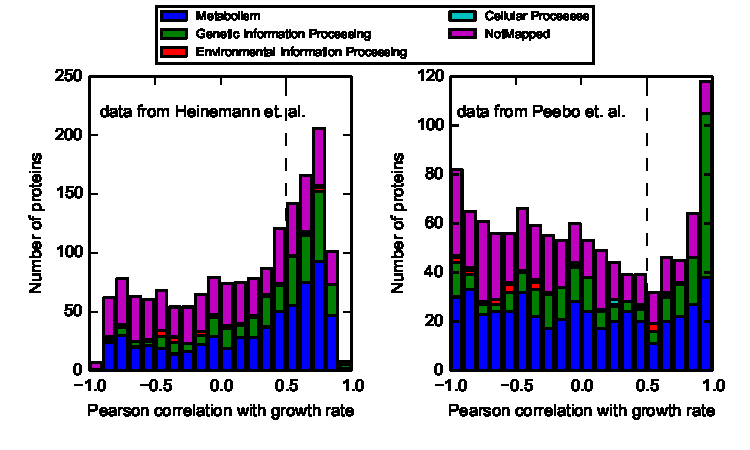
\includegraphics[width=1\columnwidth]{../GrowthRateCorrelation.pdf}
\caption{\label{fig:growthcorr}
A strong positive Pearson correlation between the fraction out of the proteome and the growth rate is observed for a large number of proteins in the two data sets analyzed (panels A and B).
Including the two fast growth conditions from the data set in \cite{Heinemann2015} in the analysis reveals down regulation of many proteins under these conditions, as is predicted by our model, recducing the number of proteins that present a strong positive Pearson correlation with the growth rate (panel C).
Thresholds used for high correlation are marked in dashed lines.
Functional groups are denoted by different colors.
Shuffling the amounts of every protein across conditions reveals the bias towards positive correlation with growth rate is a non-trivial feature of the data as is demonstrated in panel D for the data set from \cite{Peebo_2015}.
%
}
\end{center}
\end{figure}

Our model predicts that non-differentially regulated proteins should preserve their relative ratios across conditions.
We refer to such proteins as being \emph{coordinated} or \emph{coordinately regulated}.
We have shown above that many proteins are positively correlated with growth rate.
However, we note that having similar correlation with growth rate for different proteins does not imply that such proteins are coordinated, i.e. that they share the same scaling with growth rate.
Theoretically, proteins with identical correlation with growth rate may have very different slopes or fold changes with increasing growth rate.

In order to examine how similar the behavior with growth rate is for the group of strongly positively correlated proteins, we normalized each of them to its mean abundance and calculated the slope of a linear regression line for the normalized fraction vs. the growth rate.
This normalization procedure elucidates how the amount of each protein scales across different conditions, relative to its mean fraction out of the proteome.
The slopes of $\approx \frac{2}{3}$ of the proteins lie in the range $(0.5,2)$.
Which is consistent with what we expect of proteins that share a single, identical slope, but with the calculated noise in measurement for the data set from \cite{Heinemann2015} but for  the data from \cite{Peebo_2015} the expected distribution should be narrower.

Our results support the notion that a large number of proteins maintain their relative concentrations across different growth conditions and thus extend the scope of similar results obtained for \emph{S.cerevisiae} in \cite{Keren2013a} and for expression levels in \emph{E.coli} under stress conditions \cite{Kaneko2014}.
In contrast to other approaches, our model suggests a mechanism for this coordinated expression changes that is not based on shared transcription factors but rather is a result of passive redistribution of resources.

To assess the significance of the positive correlation of proteins with growth rate, out of the total change in proteome composition across conditions, we summed the fractions of all of the proteins that are strongly correlated with growth rate across the conditions measured and plotted their total fraction against the growth rate in Figure \ref{fig:globalgrcorr}.
Both data sets show that the fraction of these proteins change $\approx 2$ fold across a $\approx 5$ fold change in the growth rate under the different growth conditions.
This change is smaller than the $1:1$ change predicted by our basic model and the deviations may result from the effects of degradation and varying biosyntheis rates.
Most of the variability of the total fraction of these proteins can be explained by the growth rate ($R^2$ of $\hGlobalSumRsq$ in the data set from \cite{Heinemann2015} and $\vGlobalSumRsq$ in the data set from \cite{Peebo_2015}). 
Importantly, the strongly correlated proteins form a large fraction of the proteome, exceeding $50\%$ of the proteome by weight, at the higher growth rates.

\begin{figure}[H]
\begin{center}
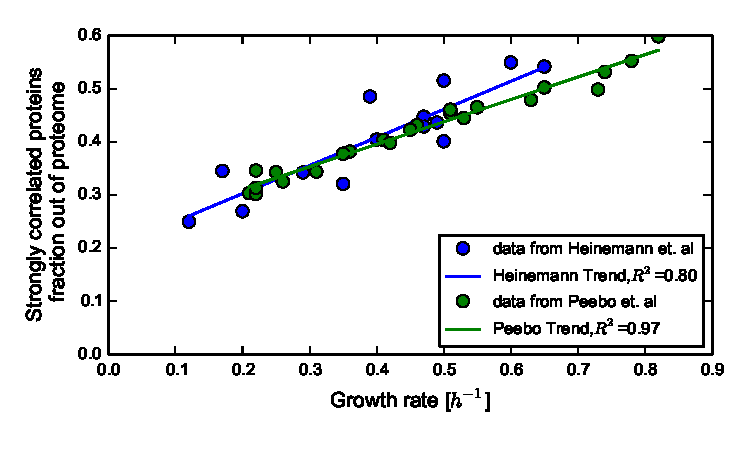
\includegraphics[width=1\columnwidth]{../GlobalClusterGRFit.pdf}
\caption{\label{fig:globalgrcorr}
Fraction of the proteome occupied by proteins that are strongly positively correlated with growth rate.
The accumulated sum of the proteins that are strongly positively correlated with growth rate (defined as having a correlation above $0.5$), as a fraction out of the proteome, with linear regression lines is shown.
These proteins form a large fraction ($\ge 50\%$) out of the proteome at higher growth rates.
The accumulated fraction of the strongly correlated proteins doubles as the growth rate changes by about 5-fold.
Assuming constant degradation rates, the trend lines correspond to protein half life times of $\approx 1.7$ hours.
Randomized data sets result in much fewer strongly positively correlated with growth rate proteins, implying a much smaller accumulated fraction (hollow circles).
%
}
\end{center}
\end{figure}

\section{Discussion}
We presented a parsimonious model connecting the fraction of proteins out of the proteome and the growth rate as an outcome of the limited bio-synthesis resources of cells. 
The notion of intrinsic affinity for expression, first presented in \cite{Maaloe1969}, and rarely used ever since, was re-introduced as a key determinant for the differences in expression of different proteins under a given growth condition.
The integration of the notion of intrinsic affinity for expression with the limited bio-synthesis capacity of cells was shown to result in a simple mechanism predicting increased fraction of many proteins with the growth rate, without assuming regulation by specific transcription factors for these proteins.

The framework we present emphasizes the importance of accounting for global factors, that are reflected in the growth rate, when analyzing gene expression and proteomics data, as was noted before \cite{Maaloe1969,Brauer2008,Klumpp2009,Klumpp2014,Scott2010,Berthoumieux2013,Keren2013,Gerosa2013,Valgepea2013,Hui_2015,Peebo_2015,Wei_e_2015}.
Specifically, we suggest that the default response of a protein (that is, the change in the observed expression of a protein, given that no specific regulation was applied to it) is to linearly increase with growth rate.
We point out that, as non-differentially regulated proteins maintain their relative abundances, one can deduce the parameters of the linear increase with growth rate of any non-differentially regulated protein by observing the scaling of other such proteins and fixing the ratio between the protein of interest and the reference proteins.

Interestingly, our model suggests that a linear correlation between ribosomal proteins and the growth rate might be achieved without special control mechanisms.
Nonetheless, many such mechanisms have been shown to exist \cite{Nomura1984,25149558}.
We stress that the existence of such mechanisms does not contradict the model.
Mechanisms for ribosomal proteins expression control may still be needed to achieve faster response under changing environmental conditions or a tighter regulation to avoid unnecessary production and reduce translational noise.
Furthermore, such mechanisms may be crucial for synchronizing the amount of rRNA with ribosomal proteins as the two go through different bio-synthesis pathways.
Nevertheless, the fact that many non-ribosomal proteins share the same response as ribosomal proteins do, poses interesting questions regarding the scope of such control mechanisms, their necessity and the trade-offs involved in their deployment.

The findings in this study support and broaden the findings in other recent studies.
Specifically, for \emph{S.cerevisiae} a few recent studies found that the concentration of the majority of the proteins is coordinated across conditions and increases with growth rate \cite{Keren2013a,Gasch2000,Brauer2008a}.
In principle, the model we suggest here can be applied to any exponentially growing population of cells and may thus also serve as a potential explanation for the phenomena observed in these studies and others.

Other recently published studies in \emph{E.coli} have suggested different models and in some cases have results  and predictions that do not coincide with those presented in this study.
Notably, in \cite{Klumpp2009,Klumpp2014} a decreased protein concentration for unregulated genes is predicted.
A few differences can explain this seeming discrepancy.
The modeling in \cite{Klumpp2009} relies on data collected under higher growth rates than those available in the data sets analyzed here.
The predictions of the model are based on the deduced dependence of various bio-synthesis process rates and physiological properties of the cells on the growth rate, properties that are, in turn, used to calculate the expected protein concentration for unregulated proteins under the different growth rates.
The model in \cite{Klumpp2009} refers to protein concentration and not to protein fraction out of the proteome. These quantities may differ due to changes in the ratio of total protein mass to cell dry weight, or cell volume, as a function of the growth rate.
Thus, this approach is markedly different than the approach we take, which assumes relatively small changes in bio-synthetic rates as a function of growth rate and focuses on the limited bio-synthesis resources as the main driver of changes in the resulting fraction of proteins out of the proteome.
As the model in \cite{Klumpp2009} was only tested against a handful of proteins, further data collection is required to decide which of the two models better describes the global effects of growth rate on proteome composition.

The expected availability of increasing amounts of whole proteome data sets, with higher accuracy levels, will enable further investigation of the details of cellular resource distribution.
With our model serving as a baseline, the analysis of such future data sets will shed more light on the relative roles of carefully tuned response mechanisms versus global, passive effects in shaping the proteome composition under different growth environments.


\section{Acknowledgments}
We kindly thank Matthias Heinemann for making proteomics data available before publication.
We thank Uri Alon, Stephan Klumpp, Arren Bar Even, Avi Flamholz, Elad Noor, Kaspar Valgepea, Karl Peebo and Katja Tummler for fruitful discussions and enlightening comments on this work.
This work was funded by the European Research Council (Project SYMPAC 260392); Dana and Yossie Hollander; Helmsley Charitable Foundation; Israel Ministry of Science; The Larson Charitable Foundation.
R.M. is the Charles and Louise Gartner professional chair and an EMBO young investigator program member

\bibliography{converted_to_latex.bib}
\end{document}

